\usetikzlibrary{arrows.meta,calc,fadings,patterns}
\begin{frame}{transmitting a signal}
    \begin{itemize}
    \item can vary\ldots
        \begin{itemize}
        \item voltage
        \item radio/light intensity 
        \item radio/light frequency
        \item \ldots
        \end{itemize}
    \end{itemize}
\begin{tikzpicture}
\tikzset{
    axis/.style={draw,ultra thick,-Latex},
    signal/.style={draw,very thick,violet},
    axis label/.style={draw,thin,font=\small},
},
\begin{pgfonlayer}{fg}
    \draw[axis] (0, 0) -- (0, 3);
    \draw[axis] (0, 0) -- (14, 0);
\end{pgfonlayer}
\draw[axis label] (0, .3) -- ++ (-.2, 0) node[left] {low};
\draw[axis label] (0, 2.1) -- ++ (-.2, 0) node[left] {high};
\begin{scope}
    \clip (0, 0) rectangle (14, 3);
    %\begin{scope}[yshift=.3cm,y=1.8cm]
    %\draw[signal] (0, 0) -- (3, 0) -- (3, 1) -- (5, 1) -- (5, 0) -- (9, 0) -- (9, 1) -- (11, 1) -- (11, 0) -- (16, 0);
    %\end{scope}
    \begin{scope}[yshift=.3cm,y=0.6cm]
    \draw[signal] (0, 0) -- (3, 0) -- (3, 1) -- (5, 1) -- (5, 3) -- (9, 3) -- (9, 1) -- (11, 1) -- (11, 2) --
        (13, 2) -- (13, 0) -- (15, 0);
    \end{scope}
    \fill[white,path fading=west] (12, 0) rectangle (13.8, 3);
    \fill[white] (13.8, 0) rectangle (14, 3);
\end{scope}
\end{tikzpicture}
\end{frame}

\begin{frame}{some simplifying assumptions}
    \begin{itemize}
    \item signal low/high --- no in between
    \item only one `channel' 
        \begin{itemize}
        \item won't have multiple wires/antennas/frequencies/etc.
        \item won't modulate different things same time
        \end{itemize}
    \item want to send receive bits (0 or 1)
    \end{itemize}
\begin{tikzpicture}
\tikzset{
    axis/.style={draw,ultra thick,-Latex},
    signal/.style={draw,very thick,violet},
    axis label/.style={draw,thin,font=\small},
},
\begin{pgfonlayer}{fg}
    \draw[axis] (0, 0) -- (0, 3);
    \draw[axis] (0, 0) -- (14, 0);
\end{pgfonlayer}
\draw[axis label] (0, .3) -- ++ (-.2, 0) node[left] {low};
\draw[axis label] (0, 2.1) -- ++ (-.2, 0) node[left] {high};
\begin{scope}
    \clip (0, 0) rectangle (14, 3);
    \begin{scope}[yshift=.3cm,y=1.8cm]
    \draw[signal] (0, 0) -- (3, 0) -- (3, 1) -- (5, 1) -- (5, 0) -- (9, 0) -- (9, 1) -- (11, 1) -- (11, 0) -- (16, 0);
    \end{scope}
    \fill[white,path fading=west] (12, 0) rectangle (13.8, 3);
    \fill[white] (13.8, 0) rectangle (14, 3);
\end{scope}
\end{tikzpicture}
\end{frame}

\begin{frame}{clocking}
\begin{tikzpicture}
\tikzset{
    axis/.style={draw,ultra thick,-Latex},
    signal/.style={draw,very thick,violet},
    axis label/.style={draw,thin,font=\small},
    value/.style={font=\tt},
},
\begin{pgfonlayer}{fg}
    \draw[axis] (0, 0) -- (0, 3);
    \draw[axis] (0, 0) -- (14, 0);
\end{pgfonlayer}
\draw[axis label] (0, .3) -- ++ (-.2, 0) node[left] {low};
\draw[axis label] (0, 2.1) -- ++ (-.2, 0) node[left] {high};
\begin{scope}
    \clip (0, 0) rectangle (14, 3);
    \begin{scope}[yshift=.3cm,y=1.8cm]
    \draw[signal] (0, 0) -- (2.85, 0) -- (2.85, 1) -- (5.05, 1) -- (5.05, 0) -- (9.05, 0) -- (9.05, 1) -- (11.1, 1) -- (11.1, 0) -- (16, 0);
    \end{scope}
    \fill[white,path fading=west] (12, 0) rectangle (13.8, 3);
    \fill[white] (13.8, 0) rectangle (14, 3);
\end{scope}
\begin{visibleenv}<2,5>
\begin{scope}[yshift=-.8cm,xshift=1cm,x=2cm]
\foreach \x/\v in {0/0,1/1,2/0,3/0,4/1,5/0,6/0} {
    \draw[thick,dotted] (\x, -0.5) -- ++(0, 4.5cm);
    \node[value,anchor=north] at (\x+0.5, 0) {\v};
}
\end{scope}
\end{visibleenv}
\begin{visibleenv}<4,5>
\begin{scope}
\clip[overlay] (0, -10) rectangle (15, 10);
\begin{scope}[yshift=-.2cm,xshift=1.35cm,x=1.6cm]
\foreach \x/\v in {-1/0,0/0,1/1,2/0,3/0,4/0,5/1,6/0,7/0,8/0} {
    \draw[thick,dashed] (\x, -.5) -- ++(0, 4cm);
    \node[value,anchor=north] at (\x+0.5, 0) {\v};
}
\end{scope}
\end{scope}
\end{visibleenv}
\begin{visibleenv}<3,5>
\begin{scope}[yshift=-1.3cm,xshift=1cm,x=1cm]
\foreach \x/\v in {0/0,1/0,2/1,3/1,4/0,5/0,6/0,7/0,8/1,9/1,10/0,11/0} {
    \draw[thick,dashed] (\x, -.5) -- ++(0, 5cm);
    \node[value,anchor=north] at (\x+0.5, 0) {\v};
}
\end{scope}
\end{visibleenv}
\end{tikzpicture}
\end{frame}

\begin{frame}{keeping a clock}
\begin{tikzpicture}
\tikzset{
    axis/.style={draw,ultra thick,-Latex},
    signal/.style={draw,very thick,violet},
    axis label/.style={draw,thin,font=\small},
    value/.style={font=\tt},
},
\begin{pgfonlayer}{fg}
    \draw[axis] (0, 0) -- (0, 3);
    \draw[axis] (0, 0) -- (14, 0);
\end{pgfonlayer}
\draw[axis label] (0, .3) -- ++ (-.2, 0) node[left] {low};
\draw[axis label] (0, 2.1) -- ++ (-.2, 0) node[left] {high};
\begin{scope}
    \clip (0, 0) rectangle (14, 3);
    \begin{scope}[yshift=.3cm,y=1.8cm]
    \draw[signal] (0, 0) -- (2.85, 0) -- (2.85, 1) -- (5.05, 1) -- (5.05, 0) -- (9.05, 0) -- (9.05, 1) -- (11.1, 1) -- (11.1, 0) -- (16, 0);
    \end{scope}
    \fill[white,path fading=west] (12, 0) rectangle (13.8, 3);
    \fill[white] (13.8, 0) rectangle (14, 3);
\end{scope}

\begin{scope}[yshift=-4cm]
    \begin{pgfonlayer}{fg}
        \draw[axis] (0, 0) -- (0, 3);
        \draw[axis] (0, 0) -- (14, 0);
    \end{pgfonlayer}
    \draw[axis label] (0, .3) -- ++ (-.2, 0) node[left] {low};
    \draw[axis label] (0, 2.1) -- ++ (-.2, 0) node[left] {high};
    \begin{scope}
        \clip (0, 0) rectangle (14, 3);
        \begin{scope}[yshift=.3cm,y=1.8cm]
        \begin{visibleenv}<2->
        \draw[signal,alt=<3->{opacity=0.1}]
            (0, 1) -- (1, 1) -- (1, 0) -- (2, 0) -- (2, 1) 
        -- (2.95, 1) -- (2.95, 0) -- (4, 0) -- (4, 1) -- (5.08, 1) -- (5.08, 0)
        -- (6, 0) -- (6, 1) -- (7.05, 1) -- (7.05, 0) -- (8, 0) -- (8, 1)
        -- (8.95, 1) -- (8.95, 0) -- (10, 0) -- (10, 1) -- (11.0, 1) -- (11.0, 0)
        -- (12, 0) -- (12, 1) -- (13, 1) -- (13, 0) -- (14, 0) -- (14, 1) --(15, 1);
        \end{visibleenv}
        \begin{visibleenv}<3-4>
        \draw[signal]
            (0, 1) -- (1, 1) -- (1, 0) -- (2, 0) -- (2, 1) 
        -- (2.85, 1) edge[red] (2.85, 0) (2.85,0) -- (3.9, 0) edge[red] (3.9, 1) (3.9, 1)-- (5.05, 1) edge[red] (5.05, 0)
        (5.05, 0)
        -- (6, 0) -- (6, 1) -- (7.05, 1) -- (7.05, 0) -- (8, 0) -- (8, 1)
        -- (9.05, 1) edge[red] (9.05, 0) (9.05, 0) -- (10.05, 0) edge[red] (10.05, 1) (10.05, 1) -- (11.1, 1) edge[red] (11.1, 0) (11.0, 0)
        -- (12, 0) -- (12, 1) -- (13.1, 1) edge[red] (13.1, 0) (13.1, 0) -- (14, 0) -- (14, 1) --(15, 1);
        \end{visibleenv}
        \end{scope}
        \fill[white,path fading=west] (12, 0) rectangle (13.8, 3);
        \fill[white] (13.8, 0) rectangle (14, 3);
    \end{scope}
\end{scope}
\begin{visibleenv}<2->
    \begin{scope}[yshift=-.2cm,xshift=1cm,x=2cm]
    \foreach \x/\v in {0/0,1/1,2/0,3/0,4/1,5/0,6/0} {
        \node[value,anchor=north] at (\x+0.5, 0) {\v};
    }
    \end{scope}
    \begin{scope}[yshift=-.2cm]
    \foreach \loc in {1,2.95,5.08,7.05,8.95,11,13,15} {
        \draw[thick,dashed] (\loc, -4) -- ++(0, 7);
    }
    \end{scope}
\end{visibleenv}
\begin{visibleenv}<3-4>
    \begin{scope}[yshift=-.2cm]
    \tikzset{
        marked/.style={red,ultra thick},
    }
    \foreach \loc/\mark in {1/,2.85/marked,5.05/marked,7.05/,9.05/marked,11.1/marked,13.1/marked,15.1/} {
        \draw[thick,dashed,\mark] (\loc, -4) -- ++(0, 7);
    }
    \end{scope}
\end{visibleenv}
\end{tikzpicture}
\end{frame}

\begin{frame}{self-synchronizing?}
    \begin{itemize}
    \item can resynchronize clock by looking for transitions
    \item but doesn't work if lots of consecutive 0s or 1s
    \vspace{.5cm}
    \item also, need to know where low and high point is
    \item important to have transitions to low/high to calibrate this
    \end{itemize}
\end{frame}

\begin{frame}{Manchester encoding}
\begin{tikzpicture}
\node (fig) { 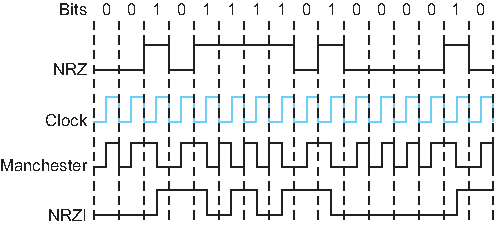
\includegraphics[width=0.9\textwidth]{../physical/SysApproach-2-Fig-25.pdf} };
\end{tikzpicture}
\imagecredit{Figure 25 from Section 2.2 of \textit{Computer Networks: A Systems Approach} (6th ed) (Peterson and Davie)}
\end{frame}

\begin{frame}{problem with Manchester}
    \begin{itemize}
    \item fixed the problem of too few transitions
    \vspace{.5cm}
    \item but now most transitions don't send information
    \item means we aren't making goo duse of wire/etc. capacity
    \vspace{.5cm}
    \item there are more clever compromises
        \begin{itemize}
        \item (example: 4B5B encoding)
        \end{itemize}
    \end{itemize}
\end{frame}

\begin{frame}{other better encoding options}
    \begin{itemize}
    \item vary more than just one thing
        \begin{itemize}
        \item example: pulse amplitude and duration
        \end{itemize}
    \item use more than just low/high
    \item \ldots much more
    \vspace{.5cm}
    \item probably covered in ECE Signals course?
    \end{itemize}
\end{frame}
